%%%%%%%%%%%%%%%%%%%%%%%%%%%%%%%%%%%%%%%%%%%%%%%%%%%
% CHƯƠNG 1: TỔNG QUAN ĐỀ TÀI
%%%%%%%%%%%%%%%%%%%%%%%%%%%%%%%%%%%%%%%%%%%%%%%%%%%
\section*{CHƯƠNG 1. TỔNG QUAN ĐỀ TÀI}
\addcontentsline{toc}{section}{\numberline{}CHƯƠNG 1. TỔNG QUAN ĐỀ TÀI}
\setcounter{section}{1}
\setcounter{subsection}{0}
\setcounter{figure}{0}
\setcounter{table}{0}

\subsection{Đặt vấn đề và Ý nghĩa thực tiễn}

Trong những năm gần đây, sự bùng nổ của cuộc Cách mạng Công nghiệp 4.0 với các công nghệ mũi nhọn như Trí tuệ nhân tạo (AI), Dữ liệu lớn (Big Data), Điện toán đám mây (Cloud Computing) và Internet vạn vật (Internet of Things -- IoT) đã tạo nên những thay đổi mang tính cách mạng trong mọi lĩnh vực đời sống. Trong ngành y tế, xu hướng chuyển đổi số y khoa (Digital Health) đang diễn ra mạnh mẽ nhằm tối ưu hóa quy trình khám chữa bệnh và nâng cao chất lượng chăm sóc sức khỏe cộng đồng. Sự giao thoa giữa công nghệ IoT và y sinh học đã hình thành nên khái niệm Internet của các thiết bị y tế (Internet of Medical Things -- IoMT). Đây là hệ thống kết nối các thiết bị y tế chuyên dụng, các cảm biến đeo trên cơ thể (Wearable Sensors) với hạ tầng mạng Internet để thu thập, truyền tải và phân tích dữ liệu sức khỏe người dùng một cách liên tục, tự động và theo thời gian thực. Công nghệ này đang dần định hình lại mô hình y tế truyền thống, chuyển dịch từ trạng thái "y tế bị động" (bệnh nhân chỉ đến bệnh viện khi có triệu chứng lâm sàng rõ rệt) sang "y tế chủ động" (giám sát liên tục từ xa nhằm phát hiện sớm các nguy cơ bệnh lý ngay tại gia đình).

Theo các báo cáo dịch tễ học chính thức của Tổ chức Y tế Thế giới (WHO), các bệnh lý không lây nhiễm (NCDs), đặc biệt là bệnh lý về tim mạch và đường hô hấp, vẫn luôn là nguyên nhân gây tử vong hàng đầu trên toàn cầu. Mỗi năm, các bệnh lý tim mạch cướp đi sinh mạng của khoảng 17,9 triệu người, chiếm đến 31\% tổng số ca tử vong toàn cầu. Tại Việt Nam, theo thống kê của Bộ Y tế, tỷ lệ tử vong do bệnh tim mạch chiếm khoảng 33\% tổng số ca tử vong hằng năm, cao hơn cả gánh nặng của các bệnh lý ung thư. Đặc biệt, sau đại dịch COVID-19, nhận thức của xã hội về vai trò sống còn của nồng độ bão hòa oxy trong máu ($SpO_2$) và thân nhiệt đã được nâng cao rõ rệt. $SpO_2$ được coi là "sinh hiệu thứ 5" cực kỳ quan trọng bên cạnh nhịp tim, huyết áp, nhịp thở và nhiệt độ. Sự suy giảm $SpO_2$ dưới ngưỡng sinh lý bình thường ($<95\%$) là dấu hiệu cảnh báo sớm của tình trạng thiếu oxy mô, suy hô hấp cấp tính hoặc hội chứng "thiếu oxy thầm lặng" (Happy Hypoxia) -- một hiện tượng nguy hiểm khi người bệnh bị suy giảm oxy máu nghiêm trọng nhưng không có cảm giác khó thở rõ rệt, dẫn đến tử vong đột ngột nếu không được phát hiện kịp thời.

Mô hình kết nối y sinh hiện đại thông qua IoT được biểu diễn qua Hình \ref{fig:so_do_khoi_datn}. Dữ liệu từ các thiết bị đeo thông minh của bệnh nhân được đồng bộ trực tiếp lên hệ thống máy chủ API thông qua mạng Wi-Fi/Internet, cung cấp công cụ giám sát tức thì cho các y bác sĩ tại trung tâm y tế.

\begin{figure}[H]
    \centering
    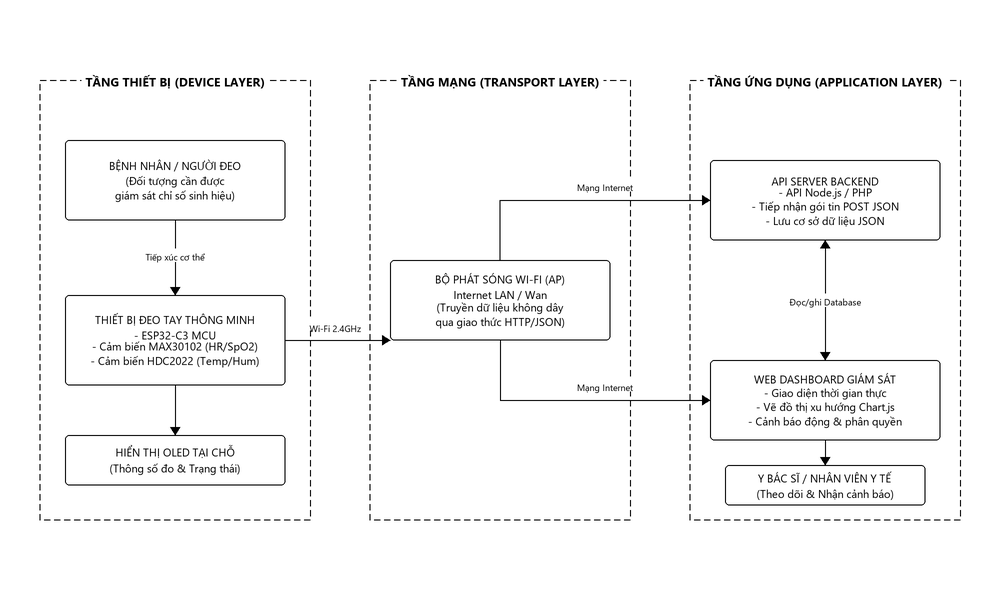
\includegraphics[width=0.95\textwidth]{images/mo_hinh_iot.png}
    \caption[Mô hình tổng quát ứng dụng IoT trong giám sát y sinh từ xa]{\bfseries\fontsize{12pt}{0pt}\selectfont Mô hình tổng quát ứng dụng IoT trong giám sát y sinh từ xa}
    \label{fig:so_do_khoi_datn}
\end{figure}

Việc theo dõi liên tục bốn chỉ số sinh hiệu cơ bản bao gồm nhịp tim, nồng độ bão hòa oxy trong máu ($SpO_2$), nhiệt độ da và độ ẩm cơ thể đóng vai trò quyết định giúp phát hiện sớm các trạng thái lâm sàng nguy kịch như suy hô hấp cấp, nhồi máu cơ tim, sốt cao co giật hay rối loạn tuần hoàn ngoại vi. Điều này đặc biệt có ý nghĩa đối với nhóm đối tượng có nguy cơ cao như người cao tuổi sống neo đơn, bệnh nhân mắc bệnh tim mạch/hô hấp mãn tính (như COPD, hen suyễn) cần được theo dõi liên tục sau khi xuất viện, hoặc quản lý tập trung các chỉ số sinh hiệu của hàng trăm bệnh nhân nội trú tại các cơ sở y tế mà không làm quá tải đội ngũ điều dưỡng, y tá.

\subsection{Tính cấp thiết của đề tài}

Nhu cầu theo dõi sức khỏe cá nhân và quản lý bệnh nhân từ xa đang ngày càng trở nên cấp thiết hơn bao giờ hết. Sự xuất hiện của các thiết bị đeo tay thông minh thương mại (như Apple Watch, Samsung Galaxy Watch, Garmin) đã phần nào đáp ứng nhu cầu theo dõi sức khỏe cá nhân. Tuy nhiên, việc áp dụng các thiết bị thương mại này vào hệ thống y tế công lập và các bệnh viện tại Việt Nam hiện nay đang gặp phải những rào cản rất lớn, bao gồm:
\begin{itemize}
    \item \textbf{Chi phí đầu tư quá cao:} Các thiết bị đeo thương mại tích hợp cảm biến đo sinh hiệu đạt độ chính xác y tế thường có giá thành dao động từ 5 triệu đến trên 15 triệu đồng cho một thiết bị. Việc trang bị đồng loạt các thiết bị này cho hàng trăm hoặc hàng ngàn bệnh nhân nội trú tại các bệnh viện công lập là một bài toán kinh tế bất khả thi đối với ngân sách y tế hiện nay.
    \item \textbf{Cơ chế quản lý và lưu trữ dữ liệu khép kín (Walled Garden):} Dữ liệu sức khỏe của người dùng được lưu trữ khép kín trên máy chủ đám mây riêng của các hãng công nghệ lớn (Apple Cloud, Samsung Cloud). Các nhà sản xuất này không cung cấp các API mở miễn phí và thời gian thực để các bệnh viện có thể kết xuất trực tiếp dòng dữ liệu thô (raw data) đồng bộ vào hệ thống thông tin quản lý bệnh viện (HIS -- Hospital Information System) hoặc bệnh án điện tử (EMR -- Electronic Medical Record). Điều này ngăn cản khả năng phân tích dữ liệu chuyên sâu của các bác sĩ điều trị.
    \item \textbf{Sự hạn chế về tùy biến cấu hình và an toàn thông tin:} Các thiết bị thương mại được thiết kế hướng tới người dùng cá nhân phổ thông nên không hỗ trợ cấu hình tùy chỉnh địa chỉ IP máy chủ nhận tin theo mạng LAN nội bộ của từng bệnh viện. Hơn nữa, việc gửi dữ liệu sức khỏe nhạy cảm của công dân Việt Nam lên các máy chủ đặt tại nước ngoài tiềm ẩn nhiều nguy cơ về bảo mật thông tin và vi phạm các quy định pháp lý về chủ quyền dữ liệu sức khỏe quốc gia.
    \item \textbf{Thiếu khả năng cảnh báo lâm sàng thích ứng:} Các thiết bị thương mại thường chỉ đưa ra cảnh báo dựa trên các ngưỡng sinh học chung cho mọi đối tượng. Trong môi trường bệnh viện, mỗi bệnh nhân có một bệnh lý nền khác nhau đòi hỏi các ngưỡng cảnh báo động (dynamic thresholds) được thiết lập riêng biệt bởi bác sĩ điều trị (ví dụ: ngưỡng nhịp tim cảnh báo của bệnh nhân suy tim sẽ khác với người bình thường).
\end{itemize}

Xuất phát từ những đòi hỏi khách quan trên, việc tự nghiên cứu, thiết kế và chế tạo một hệ thống giám sát sức khỏe IoT thời gian thực từ phần cứng bo mạch (bo mạch đeo tay nhỏ gọn, tích hợp sạc pin Lithium an toàn), phần mềm nhúng (Firmware xử lý tín hiệu số DSP khử nhiễu trực tiếp) cho đến máy chủ lưu trữ API và Dashboard Web giám sát chuyên dụng là một nhiệm vụ khoa học có tính cấp thiết và giá trị thực tiễn cao. Đề tài không chỉ giải quyết bài toán độc lập công nghệ, tối ưu hóa chi phí thiết bị mà còn đảm bảo tính an toàn, bảo mật và toàn vẹn dữ liệu y tế của bệnh viện.

\subsection{Mục tiêu nghiên cứu}

\begin{enumerate}
    \item \textbf{Nghiên cứu lý thuyết y sinh học}: Tìm hiểu sâu sắc về cơ sở y sinh của các chỉ số sinh hiệu cơ bản (nhịp tim, $SpO_2$, thân nhiệt, độ ẩm da) và nguyên lý đo thể tích đồ quang học PPG (Photoplethysmography) dựa trên định luật Beer-Lambert về sự hấp thụ ánh sáng của huyết sắc tố.
    \item \textbf{Thiết kế và chế tạo phần cứng}: Thiết kế sơ đồ nguyên lý và thiết kế mạch in PCB 2 lớp dạng bát giác tối ưu kích thước ($\approx 42\text{mm}$) phù hợp vỏ đồng hồ đeo tay. Tích hợp vi điều khiển thế hệ mới ESP32-C3, cảm biến sinh trắc học MAX30102, cảm biến nhiệt ẩm HDC2022, màn hình OLED SSD1306 và khối nguồn pin sạc Lithium 3.7V tích hợp mạch quản lý bảo vệ an toàn (TP4056 + DW01A + FS8205A).
    \item \textbf{Phát triển phần mềm nhúng (Firmware)}: Lập trình vi điều khiển ESP32-C3 thực hiện thu thập dữ liệu từ các cảm biến qua bus I2C. Xây dựng bộ lọc số DSP bao gồm bộ lọc khử trôi dòng DC (EMA) và lọc thông thấp số IIR để lọc nhiễu tín hiệu PPG. Triển khai giải thuật Phát hiện Đỉnh thích ứng động (Adaptive Peak Detection) để tính nhịp tim thời gian thực.
    \item \textbf{Giải quyết bài toán suy giảm tín hiệu ở cổ tay}: Nghiên cứu và thực thi giải thuật bù sai số tĩnh thích ứng đo ở cổ tay (Wrist Offset Compensation) để co dãn dữ liệu $SpO_2$ về đúng dải sinh lý chuẩn sinh học.
    \item \textbf{Tối ưu hóa kết nối và năng lượng}: Thiết kế cơ chế Captive Portal cấu hình mạng Wi-Fi và thông số máy chủ không dây thông minh qua AP Mode. Cấu hình giảm công suất phát sóng Wi-Fi (WiFi TX Power) về mức thích hợp để loại bỏ lỗi sụt dòng gây reset chip.
    \item \textbf{Xây dựng hạ tầng máy chủ trung tâm}: Thiết kế hệ thống API Server song song trên nền tảng Node.js (phục vụ kết nối phi luồng tốc độ cao) và PHP (phục vụ triển khai nhanh trên các host phổ thông), lưu trữ dữ liệu dạng tệp phẳng JSON cục bộ kết hợp ghi không đồng bộ để tối ưu tốc độ ghi đè.
    \item \textbf{Xây dựng Dashboard giám sát trực quan}: Phát triển giao diện Web Dashboard theo phong cách Dark Mode hiện đại hiển thị thời gian thực các chỉ số sinh hiệu thông qua kỹ thuật AJAX Polling, vẽ đồ thị lịch sử sinh động bằng thư viện Chart.js và tích hợp cơ chế phân quyền quản trị (Bác sĩ/Y tá) dựa trên Session Cookie.
\end{enumerate}

\subsection{Giới hạn đề tài và Bố cục báo cáo}

\textbf{Giới hạn đề tài:} 
Do giới hạn về mặt thời gian thực nghiệm và điều kiện trang thiết bị đo kiểm y tế chuyên dụng, đề tài có một số giới hạn nghiên cứu sau:
\begin{itemize}
    \item Bo mạch thiết kế dừng lại ở mức mô hình thử nghiệm nghiên cứu khoa học và chế tạo mẫu thử (Prototype), chưa trải qua quy trình kiểm nghiệm lâm sàng nghiêm ngặt của Bộ Y tế để được cấp phép sử dụng như một thiết bị y tế chuyên nghiệp.
    \item Thuật toán đo nhịp tim và $SpO_2$ hoạt động ổn định nhất khi người đeo ở trạng thái đứng yên hoặc vận động nhẹ (tĩnh tại). Đề tài chưa giải quyết triệt để vấn đề khử nhiễu động mạnh (Motion Artifacts) do các hoạt động chạy nhảy hoặc thay đổi tư thế đột ngột gây ra, vì việc này đòi hỏi cảm biến gia tốc chuyển động IMU 6 trục và thuật toán lọc thích ứng Kalman phức tạp hơn.
\end{itemize}

\textbf{Bố cục báo cáo:} 
Báo cáo tốt nghiệp được cấu trúc chặt chẽ thành 6 chương nội dung chính:
\begin{itemize}
    \item \textbf{Chương 1: Tổng quan đề tài} -- Trình bày đặt vấn đề, ý nghĩa thực tiễn, tính cấp thiết, mục tiêu nghiên cứu và giới hạn của đề tài.
    \item \textbf{Chương 2: Cơ sở lý thuyết và Kiến trúc hệ thống} -- Phân tích cơ sở y sinh, nguyên lý quang học PPG, giao thức I2C, thông số kỹ thuật chi tiết của các linh kiện sử dụng, giới thiệu phần mềm Altium Designer, môi trường lập trình Arduino IDE và kiến trúc Client-Server.
    \item \textbf{Chương 3: Thiết kế và Chế tạo phần cứng thiết bị} -- Mô tả chi tiết sơ đồ nguyên lý 6 khối chức năng, quy trình thiết kế mạch in PCB 2 lớp và mô hình cơ khí 3D cho đồng hồ đeo tay.
    \item \textbf{Chương 4: Lập trình Firmware vi điều khiển ESP32-C3} -- Trình bày lưu đồ thuật toán chính, các thuật toán xử lý tín hiệu số DSP lọc sóng PPG, giải thuật phát hiện đỉnh, thuật toán bù sai số tĩnh thích ứng ở cổ tay và cơ chế cấu hình mạng Captive Portal.
    \item \textbf{Chương 5: Xây dựng Máy chủ trung tâm và Giao diện Dashboard} -- Mô tả thiết kế cơ sở dữ liệu JSON, lập trình Backend API Server (Node.js/PHP) và xây dựng giao diện Dashboard Web thời gian thực tích hợp phân quyền bảo mật.
    \item \textbf{Chương 6: Thử nghiệm thực tế và Đánh giá kết quả} -- Trình bày bảng danh mục linh kiện (BOM), quá trình thử nghiệm đo đạc thực tế, đối sánh dữ liệu đo với thiết bị y tế chuyên dụng Beurer PO30 để đánh giá sai số tuyệt đối trung bình (MAE).
\end{itemize}
